\chapter{Example Programs}
In this Chapter we will present a few small example programs that that illustrate the concepts discussed so far.

\section{Perfect Numbers}
The first example shows the computation of the \blue{perfect} numbers.  A natural number $n$ is a
\href{https://en.wikipedia.org/wiki/Perfect_number}{perfect} number if it is the sum of all its \blue{proper divisors},
where a natural number $t$ is a proper divisor of $n$ if $t$ divides $n$ evenly, i.e. iff
\\[0.2cm]
\hspace*{1.3cm}
$\texttt{mod}\; n\; t = 0$.
\\[0.2cm]
Figure \ref{fig:perfect.hs} on page \pageref{fig:perfect.hs} show a program to compute the list of all perfect
numbers.  The function \texttt{isPerfect} takes a single natural number and checks whether it is perfect, while
the function \texttt{perfect} computes the list of all perfect numbers.

\begin{figure}[!ht]
\centering
\begin{minted}[ frame         = lines, 
                 framesep      = 0.3cm, 
                 firstnumber   = 1,
                 bgcolor       = bg,
                 numbers       = left,
                 numbersep     = -0.2cm,
                 xleftmargin   = 0.8cm,
                 xrightmargin  = 0.8cm,
               ]{python3}
    isPerfect :: Integer -> Bool
    isPerfect n = sum [t | t <- [1.. n-1], mod n t == 0] == n
    
    perfect :: [Integer]
    perfect = [n | n <- [1..], isPerfect n]
\end{minted}
\vspace*{-0.3cm}
\caption{Computing the perfect numbers.}
\label{fig:perfect.hs}
\end{figure}

\section{Computing Word Frequencies}
The following example is inspired by an example from the book
\emph{Thinking Functionally with Haskell} by Richard Bird \cite{bird:2014}.
In \href{https://en.wikipedia.org/wiki/stylometry}{stylometry} one of the tasks is to compute the
relative frequencies of different words occurring in a text.  Stylometry can be used for
\blue{authorship attribution}, compare for example the book \emph{Authorship Attribution} by Patrick
Juola \cite{juola:2008}.  Figure \ref{fig:common-words.hs} on page \pageref{fig:common-words.hs}
shows a program that reads a file, in our case this file contains the text of the book \emph{Moby Dick}
by Herman Melville \cite{melville:1851} and then computes the frequencies of the hundred most common words.

\noindent
Before we can discuss the program from Figure \ref{fig:common-words.hs} we need to discuss some library
functions that we will use.
\begin{enumerate}[(a)]  
\item The \texttt{break} function in Haskell is a higher-order function from the \texttt{Prelude} module that
      is used to split a list into two parts based on a predicate. 
      The type signature of \texttt{break} is:
      \\[0.2cm]
      \hspace*{1.3cm}
      \texttt{break :: (a -> Bool) -> [a] -> ([a], [a])}
      \\[0.2cm]
      Therefore a call of this function has the form
      \\[0.2cm]
      \hspace*{1.3cm}
      \texttt{break p xs}
      \begin{itemize}
      \item The first argument \texttt{p} has type \texttt{(a -> Bool)}.  It is a \textbf{predicate} that
            determines where the list should be split. 
      \item The second argument \texttt{xs} is a list of elements of some generic type \texttt{[a]} that is to
            be split in two parts.
      \item The function satisfies the following specification:
            \begin{lstlisting}[style=haskellstyle, language=Haskell]
  break p xs = (first, second)
      where
          first = [ x | x <- xs, not (p x) ]
          first + second == xs
            \end{lstlisting}
            The return value is a pair.  The \texttt{first} component of this pair is the list of all elements
            \texttt{x} of the list \texttt{xs} that do not satisfy the predicate \texttt{p}.  The
            \texttt{second} component contains the remaining elements of \texttt{xs}.
    \end{itemize}
    For example, we have
    \\[0.2cm]
    \hspace*{1.3cm}
    \texttt{break (> 3) [1, 2, 3, 4, 5] = ([1, 2, 3], [4, 5])}
    \\[0.2cm]
    The function \texttt{break} scans the list from left to right.  It collects elements into the first list
    until the predicate function returns \texttt{True}.  The second list starts from the first element where
    the predicate \texttt{p} is satisfied.  The function \texttt{break} can be implemented as follows:
\begin{lstlisting}[style=haskellstyle, language=Haskell]
break _ [] = ([], [])  -- Base case: Empty list returns two empty lists
break p (x:xs)
    | p x       = ([], x:xs) 
    | otherwise = (x:ys, zs) 
    where (ys, zs) = break p xs
\end{lstlisting}
\item The function \texttt{sort} is part of the \texttt{Data.List} module in Haskell. It is used to sort a list
      in ascending order based on the default ordering of its elements.  It has the following type signature:
      \\[0.2cm]
      \hspace*{1.3cm}
      \texttt{sort ::\;(Ord a) => [a] -> [a]}
      \\[0.2cm]
      Given a list \texttt{xs} the expression \texttt{sort xs} returns the list \texttt{xs} sorted in ascending
      order.
    
      The function requires that the elements of the list belong to the \texttt{Ord} type class (i.e., they must
      support comparison operations).  The implementation in \texttt{Data.List} is using the
      \href{https://en.wikipedia.org/wiki/Merge_sort}{merge sort} algorithm.
\item The function \texttt{words} is part of the \texttt{Data.List} module in Haskell. It is used to split a
      string into a list of words, where words are defined as contiguous sequences of non-whitespace characters. 
      It has the following type signature:
      \\[0.2cm]
      \hspace*{1.3cm}
      \texttt{words :: String -> [String]}
      \\[0.2cm]
      Given a string \texttt{s}, the expression \texttt{words s} breaks \texttt{s} into a list of words, using
      whitespace as the delimiter.  Consecutive whitespace characters are treated as a single separator,
      meaning that empty strings between spaces are ignored.  Leading and trailing whitespace is also ignored.
      The following examples show the behaviour of the function \texttt{words}:
      \begin{itemize}
      \item \texttt{words "Hello, world!" = ["Hello,","world!"]}
      \item \texttt{words "Martin Müller-Lüdenscheid" = ["Martin","Müller-Lüdenscheid"]}
      \end{itemize}
      Note that punctuation marks like ``\texttt{,}'' or ``\texttt{!}'' are not separated from other letters.

      A simple way to implement \texttt{words} recursively is as follows:
      \begin{lstlisting}[style=haskellstyle, language=Haskell]
import Data.Char (isSpace)
words :: String -> [String]
words [] = []  -- Base case: an empty string results in an empty list
words s  = let s' = dropWhile isSpace s  -- drop leading whitespace
           in case s' of
               [] -> []  
               _  -> let (word, rest) = break isSpace s'  
                     in word : words rest  
\end{lstlisting}
      
\item The function \texttt{isAlpha} has type
      \\[0.2cm]
      \hspace*{1.3cm}
      \texttt{isAlpha ::\;Char -> Bool}
      \\[0.2cm]
      and checks, whether the given character is an \blue{alphabetic} Unicode character, i.e.~for a
      character \texttt{c} the call
      \\[0.2cm]
      \hspace*{1.3cm}
      \texttt{isAlpha c}
      \\[0.2cm]
      returns \texttt{True} if \texttt{c} is either one of the lower case letters \texttt{'a'}, $\cdots$,
      \texttt{'z'}, or of the upper case letters \texttt{'A'}, $\cdots$, \texttt{'Z'}, or a
      unicode letter from another script, like, e.g.~the Greek letter $\alpha$.            
\item The function \texttt{toLower} has the following type signature:
      \\[0.2cm]
      \hspace*{1.3cm}
      \texttt{toLower :: Char -> Char}
      \\[0.2cm]
      For a letter \texttt{c}, the expression 
      \\[0.2cm]
      \hspace*{1.3cm}
      \texttt{toLower c}
      \\[0.2cm]
      returns the lower case version of the letter \texttt{c}.  For example,
      \\[0.2cm]
      \hspace*{1.3cm}
      \texttt{toLower 'A' = 'a'} \quad and \quad \texttt{toLower 'b' = 'b'}.
\item The function \texttt{concatMap} has the type
      \\[0.2cm]
      \hspace*{1.3cm}
      \texttt{concatMap ::\;(a -> [b]) -> [a] -> [b]}
      \\[0.2cm]
      Thus, \texttt{concatMap} takes two arguments:
      \begin{itemize}
      \item A function of type \texttt{a -> [b]}, which maps each element of type \texttt{a} to a list of elements
            of type \texttt{b}. 
      \item A list of type \texttt{a}, which serves as the input to be processed.
      \end{itemize}
      The result is a single list of type \texttt{b} obtained by applying the function to each element of the
      input list and then concatenating the resulting lists. 

      The function \texttt{concatMap} can be understood as the composition of \texttt{map} and \texttt{concat}:
      \begin{itemize}
      \item \texttt{map} applies the given function to each element of the input list, producing a list of lists:
            \texttt{[a] -> [[b]]}. 
      \item \texttt{concat} then flattens this list of lists into a single list: \texttt{[[b]] -> [b]}.
      \end{itemize}
      Formally, we can express this as:
      \\[0.2cm]
      \hspace*{1.3cm}
      \texttt{concatMap f xs = concat (map f xs)}
      \\[0.2cm]
      where:
      \begin{itemize}
      \item \texttt{f} is the function of type \texttt{a -> [b]},
      \item \texttt{xs} is the input list of type \texttt{[a]}.
      \end{itemize}
      The following example shows \texttt{concatMap} at work:
      \\[0.2cm]
      \hspace*{1.3cm}
      \texttt{concatMap (\textbackslash x -> [x, x+1]) [1, 3, 5]}
      \begin{itemize}
      \item The function \texttt{\symbol{92}x -> [x, x+1]} maps each element \texttt{x} to the list \texttt{[x, x+1]}.
      \item Applying \texttt{map} yields the list of lists  \texttt{[[1, 2], [3, 4], [5, 6]]}.
      \item Applying \texttt{concat} flattens this to \texttt{[1, 2, 3, 4, 5, 6]}.
      \end{itemize}
      Thus, the result is the list
      \\[0.2cm]
      \hspace*{1.3cm}
      \texttt{[1, 2, 3, 4, 5, 6]}.   
\end{enumerate}

\begin{figure}[!ht]
\centering
\begin{minted}[ frame         = lines, 
                framesep      = 0.3cm, 
                firstnumber   = 1,
                bgcolor       = bg,
                numbers       = left,
                numbersep     = -0.2cm,
                xleftmargin   = 0.0cm,
                xrightmargin  = 0.0cm,
              ]{haskell}
    import Data.List (sort, words)
    import Data.Char (isAlpha, toLower)
    
    type Text = [Char]
    
    countRuns :: Eq a => [a] -> [(Int, a)]
    countRuns [] = []
    countRuns (x:xs) =
        let (run, rest) = break (/= x) xs
        in (1 + length run, x) : countRuns rest
    
    frequency :: Int -> Int -> Double
    frequency c n = fromIntegral c / fromIntegral n 
    
    divide :: Int -> [(Int, a)] -> [(Double, a)]
    divide n ps = [(frequency c n, x) | (c, x) <- ps]
    
    myWords :: String -> [String]
    myWords = map (filter isAlpha) . words
    
    showPair :: (Double, String) -> String 
    showPair (f, w) = w ++ ": " ++ show f ++ "\n"
    
    comnWrds :: Int -> Text -> String
    comnWrds n b = concatMap showPair $
                   divide nw . take n . reverse . sort . countRuns . sort $
                   aw
      where
        aw = (myWords . map toLower) b
        nw = length aw
                     
    readBook :: FilePath -> IO String
    readBook filename = readFile filename
    
    main :: IO ()
    main = do
        contents <- readBook "moby-dick.txt"
        putStrLn $ comnWrds 100 contents
\end{minted} 
\vspace*{-0.3cm}
\caption{Finding the most common words, \texttt{part \texttt{I}}.}
\label{fig:common-words.hs}
\end{figure} %$


We proceed to discuss the program that is shown in Figure \ref{fig:common-words.hs} on page
\pageref{fig:common-words.hs}. 
\begin{enumerate}
\item In line 1, we import the functions \texttt{sort} and \texttt{words} from the module \texttt{Data.List}. 
\item Similarly, we import \texttt{isAlpha} and \texttt{toLower} in line 2.
\item The function \texttt{countRuns} takes a sorted list of elements of type \texttt{a}
      and returns a list of pairs.  Each pair consists of a unique element from the input list
      and the count of its consecutive occurrences (runs).
      For example, we have:
      \\[0.2cm]
      \hspace*{0.8cm}
      \texttt{countRuns ['a','a','a','a','b','c','c'] = [(4,'a'),(1,'b'),(2,'c')]}
      \\[0.2cm]
      The implementation is recursive.  If the given list is non-empty and therefore has the form
      \texttt{x:xs}, we first check how often the element \texttt{x} occurs at the beginning of the list
      \texttt{xs} by breaking \texttt{xs} into two sublists:
      \begin{itemize}
      \item \texttt{run} is the longest prefix of the list \texttt{xs} that only contains the element
            \texttt{x}.
      \item \texttt{rest} is the remainder of the list \texttt{xs} after removing all occurrences of the
            element \texttt{x} from the beginning of the list \texttt{xs}.    
      \end{itemize}
      Then the element \texttt{x} occurs \texttt{1 + length run} times in the list \texttt{x:xs} because it
      occurs \texttt{length run} times in \texttt{xs} and it also is the first element of the list \texttt{x:xs}.
      Furthermore, we have to call \texttt{countRuns} recursively on the \texttt{rest} list.
\item The function \texttt{frequency} takes two natural numbers as its input.
      \begin{itemize}
      \item \texttt{c} is the number of occurrences of a given word, while
      \item \texttt{n} is the total number of words.
      \end{itemize}
      The function computes the fraction \texttt{c/n}.  It makes use of the function
      \\[0.2cm]
      \hspace*{1.3cm}
      \texttt{fromIntegral ::\;Int -> Double}
      \\[0.2cm]
      that transforms a natural number into a floating point number.  This is necessary, because division is
      only defined for floating point numbers.
\item The function \texttt{divide} is called with two arguments:
      \\[0.2cm]
      \hspace*{1.3cm}
      \texttt{divide n ps}
      \\[0.2cm]
      Here, \texttt{n} is the total number of words, while \texttt{ps} is a list of pairs of the form
      \texttt{(c, w)} where \texttt{w} is a word and \texttt{c} is the number of occurrences of this word in a
      given text.  It converts the number of occurrences into frequencies by dividing the count \texttt{c} by
      the total number of words.     
\item When we use the function \texttt{words}, the resulting words will contain punctuation symbols.  For
      example, we have
      \\[0.2cm]
      \hspace*{1.3cm}
      \texttt{words "Hello, world!" == ["Hello," ,"world!"]}
      \\[0.2cm]
      This is not what we want.  The function \texttt{myWords} takes a string, extracts the words and finally removes
      all symbols from these words that are not alphabetical characters.
\item The function \texttt{showPair} is only used to format the output.  It takes a pair of the form
      $(f, w)$ where $w$ is a word and $f$ is the frequency of this words.  It returns a string of the form 
      $\texttt{\symbol{34}}w\mathtt{:}\; f\texttt{\symbol{92}n\symbol{34}}$, where
      \texttt{\symbol{92}n\symbol{34}} is a newline symbol.
\item The function \texttt{comnWrds} is the star of the show and does the main work of extraction the word and
      computing their frequencies. The function receives two arguments
      \begin{enumerate}[(a)]
      \item \texttt{n} is the number of words that should be returned.
      \item \texttt{b} is a string representing a book.
      \end{enumerate}
      The task of the function is to return the \texttt{n} most common word from the book \texttt{b}.

      The implementation works by chaining a number of different functions together in a pipeline.
      \begin{enumerate}[(a)]
      \item The variable \texttt{aw} (short for \underline{\texttt{a}}ll \underline{\texttt{w}}ords) is a list
            containing all words.  Note that we first transform all characters in the string \texttt{b} to
            lower case before we extract the list of words.  This way, the strings ``The''  and ``the''
            represent the same word.
      \item The variable \texttt{nw}  (short for \underline{\texttt{n}}umber of \underline{\texttt{w}}ords)
            stores the number of all different words that have been found.
      \item Next, the words are sorted using the function \texttt{sort}.  This way, the same words are grouped
            together and hence it is easy to count how often each word occurs.
      \item The function \texttt{countRuns} counts the frequency of each words.  It transforms the sorted list
            of words into a list of pairs of the form
            \\[0.2cm]
            \hspace*{1.3cm}
            \texttt{[(1, "abasement"), (1, "abandonedly"), ... (981, "of"), (1073, "the"), ...]}
            \\[0.2cm]
            In these pairs, the first component is the number of occurrences of the corresponding word.
            This list is the sorted ascendingly according to the number of occurrences.  
      \item Since we want the most frequent words at the beginning, this list is reversed.
      \item Then we \texttt{take} the first \texttt{n} pairs from this list.
      \item The function \texttt{divide} turns a pair of the form
            \\[0.2cm]
            \hspace*{1.3cm}
            $(c, w)$
            \\[0.2cm]
            where $w$ is a word and $c$ is the number of occurrences of this word into a pair of the form
            \\[0.2cm]
            \hspace*{1.3cm}
            $(f, w)$
            \\[0.2cm]
            where $f$ is the frequency of the word.  This is done by dividing $c$ by the total number of all
            words \texttt{nw}.
      \item Finally, the function \texttt{concatMap} turns the list of pairs into a string with the help of the
            function \texttt{showPair}.
      \end{enumerate}      
\end{enumerate}

 
\section{The Wolf, the Goat, and the Cabbage}
Next,  we solve a problem that has puzzled the greatest agricultural economists for centuries.  The puzzle we
want to solve is known as the  
\href{http://jeux.lulu.pagesperso-orange.fr/html/anglais/loupChe/loupChe1.htm}{wolf-goat-cabbage puzzle}:  
\vspace*{0.3cm}

\begin{minipage}[c]{15cm}
{\sl
An agricultural economist has to sell a wolf, a goat, and a cabbage on a market place.  In order to
reach the market place, she has to cross a river.  The boat that she can use is so small that it can
only accommodate either the goat, the wolf, or the cabbage in addition to the agricultural economist.
Now if the agricultural economist leaves the wolf alone with the goat, the wolf will eat the goat.
If, instead, the agricultural economist leaves the goat with the cabbage, the goat will eat the cabbage.
Is it possible for the agricultural economist to develop a schedule that allows her to cross the river
without either the goat or the cabbage being eaten?
}
\end{minipage}
\vspace*{0.3cm}

\begin{figure}[!ht]
\centering
\begin{minted}[ frame         = lines, 
                 framesep      = 0.3cm, 
                 firstnumber   = 1,
                 bgcolor       = white,
                 numbers       = left,
                 numbersep     = -0.2cm,
                 xleftmargin   = -0.3cm,
                 xrightmargin  = 0.0cm,
               ]{python3}
    {-# LANGUAGE UnicodeSyntax #-}
    {-# LANGUAGE ScopedTypeVariables #-}
    module Bfs (search) where
   
    import Data.Set (Set, fromList, singleton)
    import qualified Data.Set as Set 
    
    (∪) :: Ord a ⇒ Set a → Set a → Set a
    (∪) = Set.union    
    (∈) :: (Ord a) ⇒ a → Set a → Bool
    (∈) = Set.member
    (∉) :: (Ord a) ⇒ a → Set a → Bool
    x ∉ s = not (x ∈ s)
    
    type Path a = [a]
    
    search :: forall a. Ord a ⇒ [(a, a)] → a → a → [Path a]
    search relation start goal = go [[start]] (Set.singleton start)
      where
        go :: [Path a] → Set a → [Path a]
        go [] _ = []
        go paths visited
          | null goalPaths = go newPaths newVisited
          | otherwise = goalPaths
          where
            newPaths = [ path ++ [z] | path ← paths, (y, z) ← relation, 
                                       last path == y, z ∉ visited       ]
            newVisited = visited ∪ Set.fromList [last path | path ← newPaths]
            goalPaths = filter (\p → last p == goal) newPaths
\end{minted}
\vspace*{-0.3cm}
\caption{Breadth First Search.}
\label{fig:bfs.hs}
\end{figure}


\begin{figure}[!ht]
\centering
\begin{minted}[ frame         = lines, 
                 framesep      = 0.3cm, 
                 firstnumber   = 1,
                 bgcolor       = bg,
                 numbers       = left,
                 numbersep     = -0.2cm,
                 xleftmargin   = 0.3cm,
                 xrightmargin  = 0.3cm,
               ]{haskell}
    import Data.Set (Set, (\\), fromList, toList, empty)
    import qualified Data.Set as Set
    import Bfs (search)
    import SetUtils (power, (∪), (∩), (∈), (∉))
      
    problem :: Set String -> Bool
    problem s =
        "farmer" ∉ s &&
        (("goat" ∈ s && "cabbage" ∈ s) || ("wolf" ∈ s && "goat" ∈ s))       
    
    allItems :: Set String
    allItems = fromList ["farmer", "wolf", "goat", "cabbage"]
    
    noProblem :: Set String -> Bool
    noProblem s = not (problem s) && not (problem $ allItems \\ s)
    
    states :: Set (Set String)
    states = Set.filter noProblem (power allItems)
    
    r1 :: [(Set String, Set String)]
    r1 = [ (s, diff)
         | s <- toList states
         , b <- toList $ power s
         , let diff = s \\ b 
         , diff ∈ states
         , "farmer" ∈ b
         , length b <= 2
         ]
    
    r2 :: [(Set String, Set String)]
    r2 = map (\(s1, s2) -> (s2, s1)) r1
    
    r :: [(Set String, Set String)]
    r = r1 ++ r2
    
    start = allItems
    goal  = empty
    
    path :: Maybe [Set String]
    path = search r start goal
\end{minted}
\vspace*{-0.3cm}
\caption{The wolf, the goat, and the cabbage.}
\label{fig:wolf-goat-cabbage.hs}
\end{figure}

\noindent
In order to compute a schedule, we first have to model the problem.  The various \blue{states} of the problem will
be regarded as \blue{nodes} of a directed graph and this graph will be represented as a binary relation.
To this end we define the set
\begin{verbatim}
  All = {'farmer', 'wolf', 'goat', 'cabbage'}.
\end{verbatim}
Every node will be represented as a subset \texttt{s} of the set \texttt{All}.  The idea is that the set \texttt{s}
specifies those objects that are on the left side of the river.  We assume that initially the farmer and his goods
are on the left side of the river. 
Therefore, the set of all states that are \blue{allowed} according to the specification of the problem can be defined
as the set 
\begin{verbatim}
  States = { s \in 2^{\texttt{All}} | not problem(S) and not problem(All-S) }
\end{verbatim}
Here, we have used the procedure \texttt{problem} to check whether a given set \texttt{S} has a problem,
where a problem is any situation where either the goat eats the cabbage or the wolf eats the goat.
Note that since \texttt{S} is the set of objects on the left side, the expression $\texttt{All-S}$
computes the set of objects on the right side of the river.

Formally, a set \texttt{S} of objects has a problem if both of the following conditions
are satisfied:
\begin{enumerate}
\item The farmer is not an element of \texttt{S} and
\item either \texttt{S} contains both the goat and the cabbage or \texttt{S} contains both the wolf and the goat.
\end{enumerate}
Therefore, we can implement the function \texttt{problem} as follows:
\begin{verbatim}
  def problem(S):
      return ('farmer' not in S) and             \
             (('goat' in S and 'cabbage' in S) or   # goat eats cabbage
              ('wolf' in S and 'goat'    in S)   )  # wolf eats goat
\end{verbatim}
Note that we have to use a \blue{line continuation backslash} ``\texttt{$\backslash$}''
at the end of the first line of the return statement.
We do not need a continuation backslash at the end of the second line of the return statement since
the opening parenthesis at the beginning of the second line has not yet been closed when the second line
finishes and therefore \textsl{Python} is able to figure out that the expression defined in this line is
continued in the third line.

We proceed to compute the relation \texttt{R} that contains all possible transitions between
different states.  We will compute \texttt{R} using the formula:
\\[0.2cm]
\hspace*{0.75cm}
\texttt{R = R1 + R2;}
\\[0.2cm]
Here \texttt{R1} describes the transitions that result from the farmer crossing the river from left
to right, while \texttt{R2} describes the transitions that result from the farmer crossing the river
from right to left.  We can define the relation \texttt{R1} as follows:
\begin{verbatim}
  R1 = { (S, S-B) for S in States 
                  for B in power(S)
                  if S-B in States and 'farmer' in B and len(B) <= 2
       }
\end{verbatim}
Let us explain this definition in detail:
\begin{enumerate}
\item Initially, \texttt{S} is the set of objects on the left side of the river.  Hence, \texttt{S}
      is an element of the set of all states that we have defined as \texttt{States}.
\item \texttt{B} is the set of objects that are put into the boat and that do cross the river.  Of
      course, for an object to go into the boat is has to be on the left side of the river to begin
      with.  Therefore, \texttt{B} is a subset of \texttt{S} and hence \texttt{B} is an element of the power set
      of \texttt{S}. 
\item Therefore  \texttt{S-B} is the set of objects that are left on the left side of the river after
      the boat has crossed.  Of course, the new state \texttt{S-B} has to be a state that does not
      have a problem.  Therefore, we check that the set \texttt{S-B} is an element of the set \texttt{States}.
\item Furthermore, the farmer has to be inside the boat.  This explains the condition 
      \\[0.2cm]
      \hspace*{1.3cm}
      \texttt{\symbol{39}farmer\symbol{39} in B}.
\item Finally, the boat can only have two passengers.  Therefore, we have added the condition
      \\[0.2cm]
      \hspace*{1.3cm}
      \texttt{len(B) <= 2}.
\end{enumerate}
Next, we have to define the relation \texttt{R2}.  However, as crossing the river from right to left
is just the reverse of crossing the river from left to right, \texttt{R2} is just the \blue{inverse} of
\texttt{R1}.   Hence we define:
\begin{verbatim}
  R2 = { (S2, S1) for (S1, S2) in R1 }.
\end{verbatim}
Next, the relation \texttt{R} is the union of \texttt{R1} and \texttt{R2}:
\begin{verbatim}
  R = R1 | R2.
\end{verbatim}
Finally, the start state has all objects on the left side.  Therefore, we have
\begin{verbatim}
  start = All.
\end{verbatim}
In the end, all objects have to be on the right side of the river.  That means that nothing is left
on the left side.  Therefore, we define
\begin{verbatim}
  goal = {}.
\end{verbatim}


\begin{figure}[h]
  \centering

  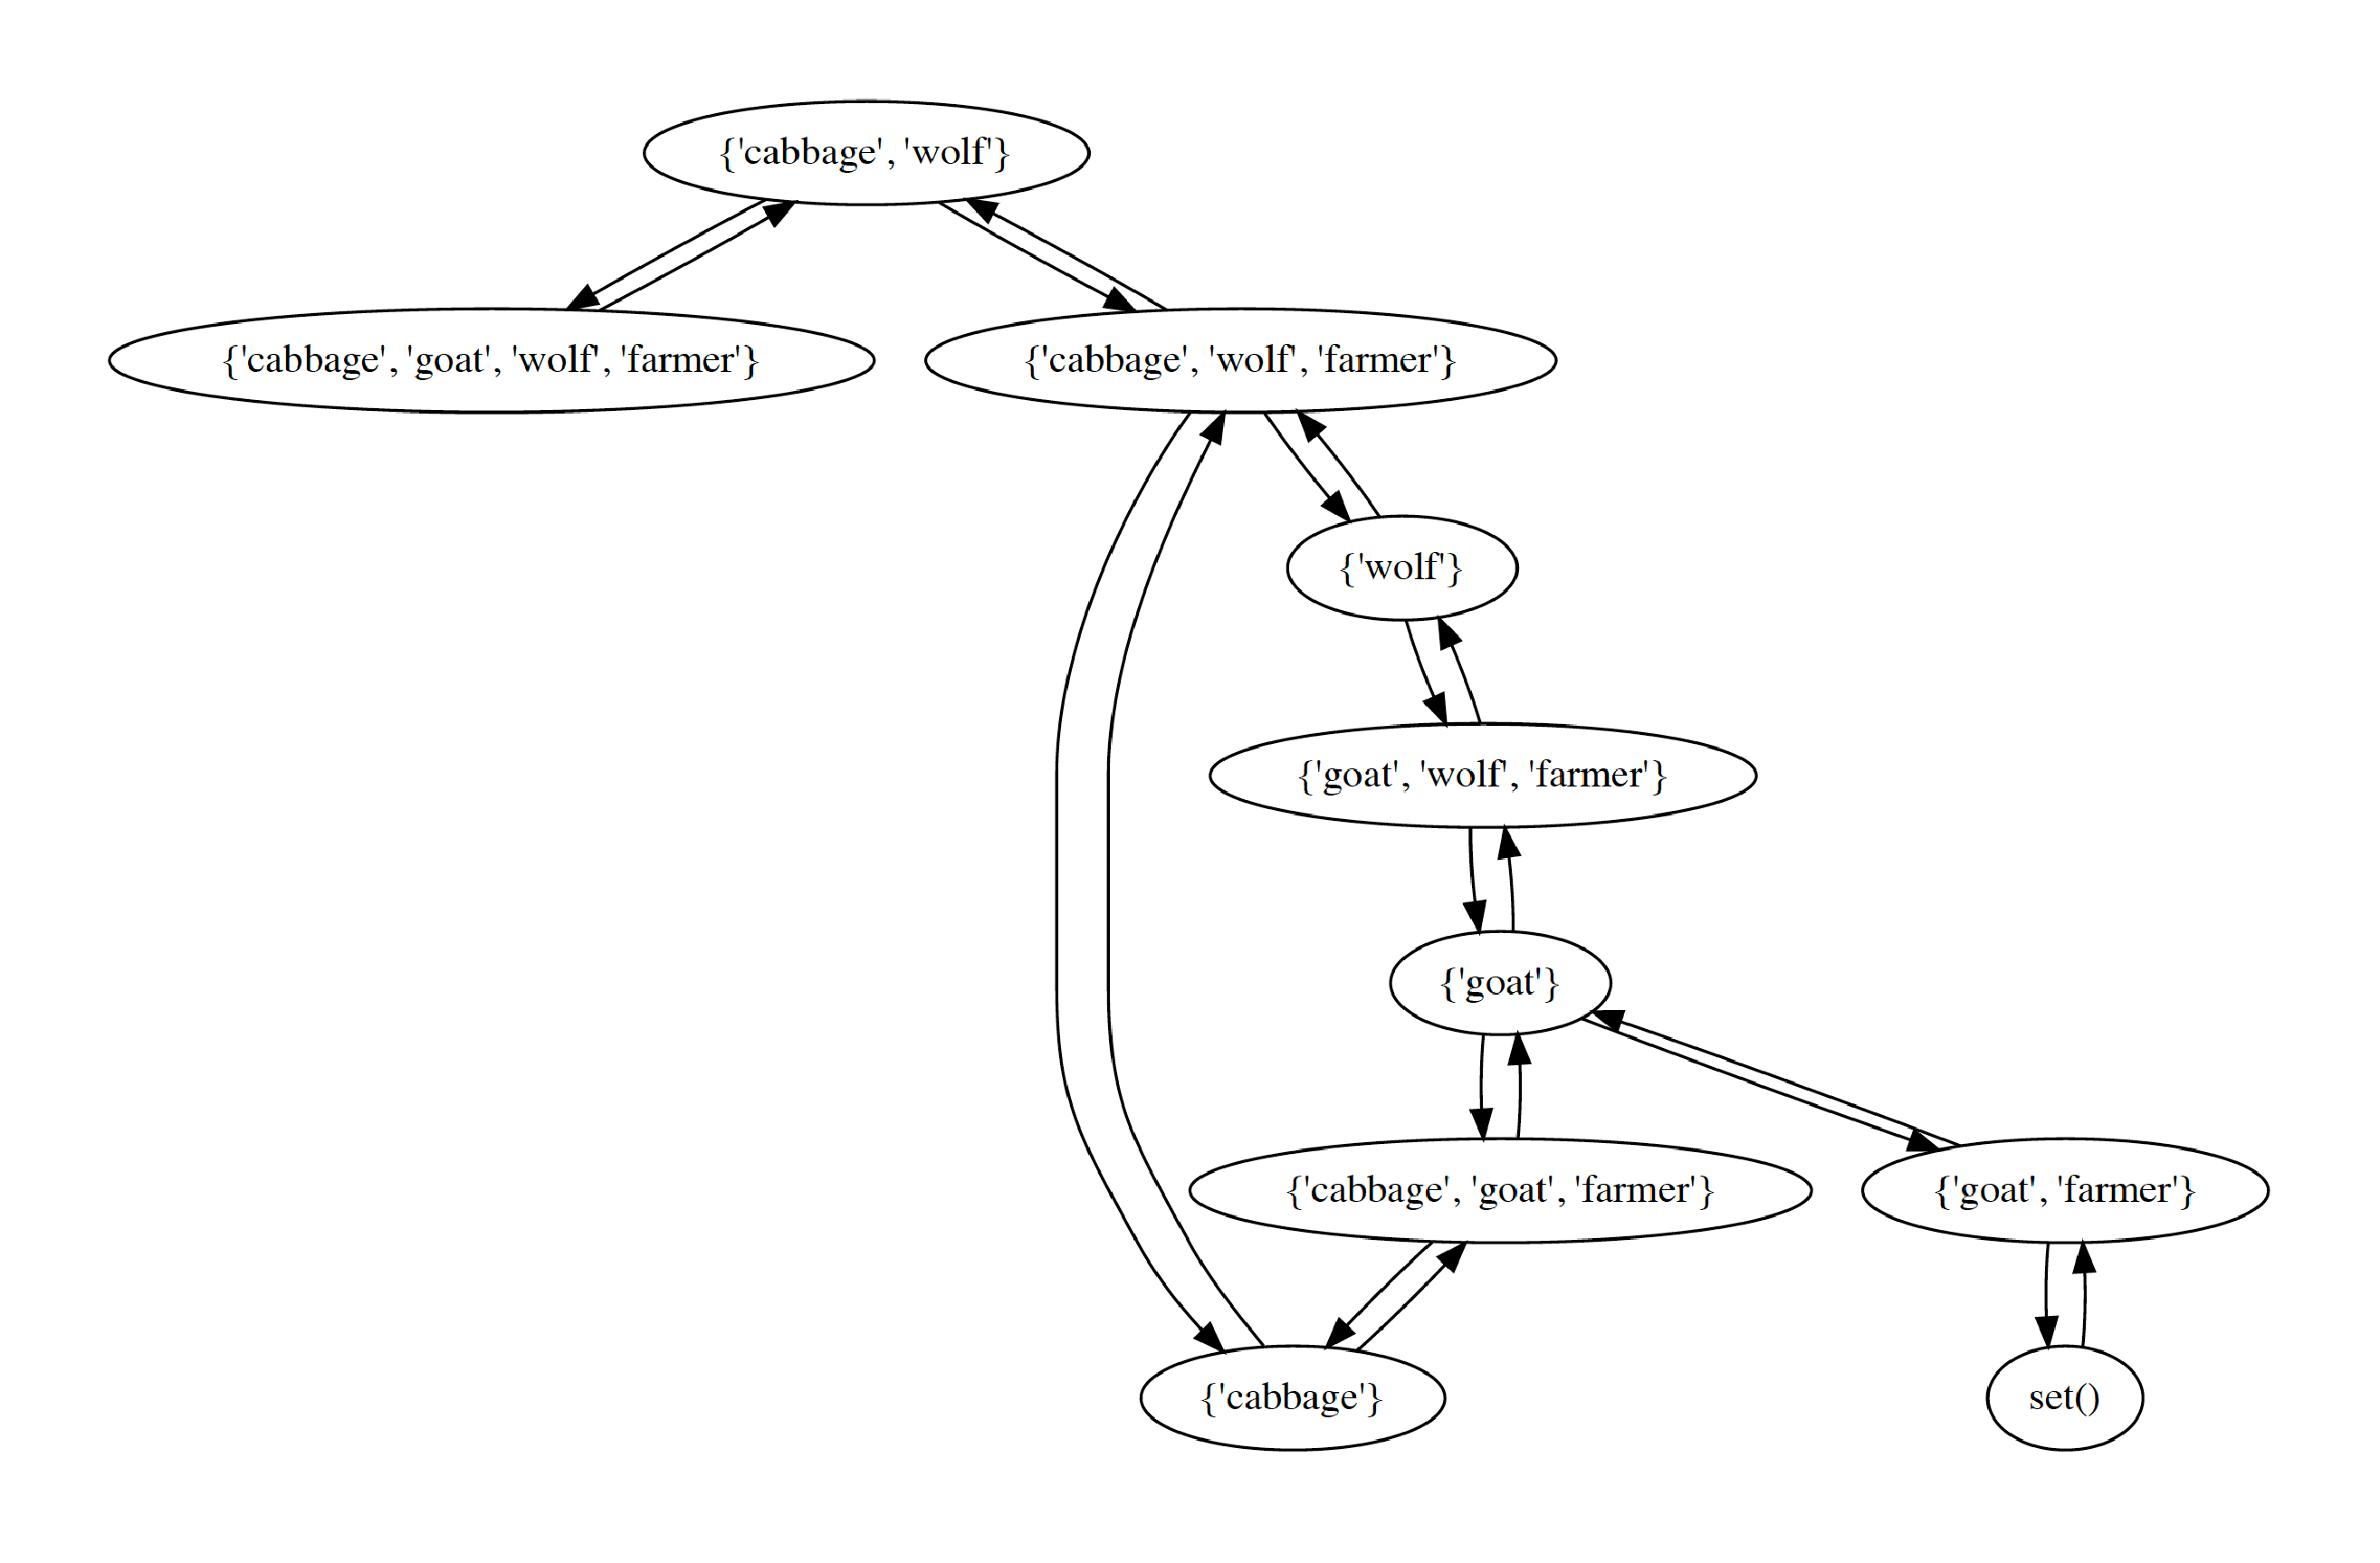
\epsfig{file=Figures/wolf-goat-cabbage, scale=0.4}

  \caption{The relation \texttt{R} shown as a directed graph.}
  \label{fig:wolf-goat-cabbage.pdf}
\end{figure}



\noindent
Figure \ref{fig:wolf-goat-cabbage.pdf} on page \pageref{fig:wolf-goat-cabbage.pdf} displays the relation $R$ graphically.
Figure \ref{fig:wolf-ziege} on page \pageref{fig:wolf-ziege} shows the program
\href{https://github.com/karlstroetmann/Logic/blob/master/Python/wolf-goat-cabbage.py}{\texttt{wolf-goat-cabbage.py}}
that combines the statements shown so far.  The solution computed by this program is shown in Figure
 \ref{fig:wolf-ziege-solution}.

\begin{figure}[!ht]
  \centering
\begin{minted}[ frame         = lines, 
                framesep      = 0.3cm, 
                numbers       = left,
                numbersep     = -0.2cm,
                bgcolor       = bg,
                xleftmargin   = 0.3cm,
                xrightmargin  = 0.3cm,
              ]{python3}
    def problem(S):
        return ('farmer' not in S) and             \
               (('goat' in S and 'cabbage' in S) or   # goat eats cabbage
                ('wolf' in S and 'goat'    in S)   )  # wolf eats goat
    
    All   = frozenset({ 'farmer', 'wolf', 'goat', 'cabbage' })
    R1    = { (S, S - B) for S in States for B in power(S)
                         if S - B in States and 'farmer' in B and len(B) <= 2
            }
    R2    = { (S2, S1) for (S1, S2) in R1 }
    R     = R1 | R2
    start = All
    goal  = frozenset()
    Path  = findPath(start, goal, R)
\end{minted} 
\vspace*{-0.3cm}
\caption{Solving the wolf-goat-cabbage problem.}  
\label{fig:wolf-ziege}
\end{figure}


\begin{figure}[!ht]
  \centering
\begin{minted}[ frame         = lines, 
                framesep      = 0.3cm, 
                numbers       = left,
                numbersep     = -0.2cm,
                bgcolor       = bg,
                xleftmargin   = 0.8cm,
                xrightmargin  = 0.8cm,
              ]{python3}
    {'cabbage', 'farmer', 'goat', 'wolf'}                                 {}
                             >>>> {'farmer', 'goat'} >>>> 
    {'cabbage', 'wolf'}                                   {'farmer', 'goat'}
                             <<<< {'farmer'} <<<< 
    {'cabbage', 'farmer', 'wolf'}                                   {'goat'}
                             >>>> {'farmer', 'wolf'} >>>> 
    {'cabbage'}                                   {'farmer', 'goat', 'wolf'}
                             <<<< {'farmer', 'goat'} <<<< 
    {'cabbage', 'farmer', 'goat'}                                   {'wolf'}
                             >>>> {'cabbage', 'farmer'} >>>> 
    {'goat'}                                   {'cabbage', 'farmer', 'wolf'}
                             <<<< {'farmer'} <<<< 
    {'farmer', 'goat'}                                   {'cabbage', 'wolf'}
                             >>>> {'farmer', 'goat'} >>>> 
    {}                                 {'cabbage', 'farmer', 'goat', 'wolf'}
\end{minted} 
\vspace*{-0.3cm}
\caption{A schedule for the agricultural economist.}  
\label{fig:wolf-ziege-solution}
\end{figure}

\vspace*{\fill}

%%% Local Variables:
%%% mode: latex
%%% TeX-master: "haskell"
%%% End:
